\documentclass[tikz,fontsize=8pt]{standalone}
\usepackage{fourier}
\usetikzlibrary{arrows.meta}
\usetikzlibrary{calc}
\tikzset{>=latex}
\definecolor{bookblue}{RGB}{0,173,239}
\definecolor{bookpink}{RGB}{236,0,140}
\definecolor{bookgreen}{RGB}{50,200,0}
\definecolor{bookbluearea}{RGB}{204,239,252}
\tikzstyle{blueline}=[draw=bookblue,line width=0.2mm]
\tikzstyle{pinkline}=[draw=bookpink,line width=0.2mm]
\tikzstyle{greenline}=[draw=bookgreen,line width=0.2mm]
\tikzstyle{blackline}=[draw=black,line width=0.2mm]
\tikzstyle{bluearea}=[fill=bookbluearea]

\usepackage{scrextend}
\changefontsizes[8pt]{8pt}
\usetikzlibrary{decorations.pathreplacing}
\begin{document}
  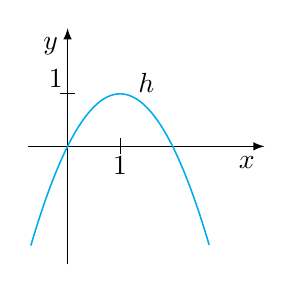
\begin{tikzpicture}
  %\node at (-0.15,-0.2) {0};
  \draw[->] (-1.5,0) -- (1.5,0) node[below left] {$x$};
  \draw[->] (-1,-1.5) -- (-1,1.5) node[below left] {$y$};
  
  \draw[blueline,domain=-0.7:2.7,samples=500] plot [smooth] ({(\x-1.5)/1.5},{(2*\x - (\x)^2)/1.5});
  \node at (-0.3334,-0.25) {$1$};
  \node at (-1.15,0.8667) {$1$};
  \node at (0,0.8) {$h$};
  \draw (-0.3334,-0.1) -- (-0.3334,0.1);
  \draw (-1.1,0.6667) -- (-0.9,0.6667);
  \end{tikzpicture}
\end{document}